\documentclass[11pt]{article}

% ------------------------------------------------------------------------------
% This is all preamble stuff that you don't have to worry about.
% Head down to where it says "Start here"
% ------------------------------------------------------------------------------

\usepackage[margin=.8in,top=1.1in,bottom=1.1in]{geometry} % page layout
\usepackage{amsmath,amsthm,amssymb,amsfonts} % math things
\usepackage{graphicx} % include graphics
\usepackage{fancyhdr} % header customization
\usepackage{titlesec} % help with section naming
\usepackage{listings}
\usepackage[final]{pdfpages}
\usepackage{pgfplots}

\pgfplotsset{compat=1.7}

% naming sections
\titleformat{\section}{\bf}{Problem \thesection}{0.5em}{}
\newcommand{\exercise}{\section{}}

% headers
\pagestyle{fancy}
\fancyhf{} % clear all
\fancyhead[L]{\sffamily\small Machine Learning 1 --- Homework}
\fancyhead[R]{\sffamily\small Page \thepage}
\renewcommand{\headrulewidth}{0.2pt}
\renewcommand{\footrulewidth}{0.2pt}
\markright{\hrulefill\quad}

\newcommand{\hwhead}[4]{
\begin{center}
\sffamily\large\bfseries Machine Learning Worksheet #1
\vspace{2mm}
\normalfont

#2\\
#3\\
\texttt{#4}
\end{center}
\vspace{6mm} \hrule \vspace{4mm}
}

% ------------------------------------------------------------------------------
% Start here -- Fill in your name, imat and email
% (and the same for who you worked with)
% You are allowed to work in groups of 2 (or 3 if there is no way around it)
% However, you each must submit individually - (it may be same file)
% ------------------------------------------------------------------------------

\newcommand{\names}{Tomas Ladek, Michael Kratzer} %
\newcommand{\imats}{3602673, 3612903} %
\newcommand{\emails}{tom.ladek@tum.de, mkratzer@mytum.de} %

\begin{document}

% ------------------------------------------------------------------------------
% Change xx (and only xx) to the current sheet number
% ------------------------------------------------------------------------------
\hwhead{6}{\names}{\imats}{\emails}

% ------------------------------------------------------------------------------
% Fill in your solutions
% ------------------------------------------------------------------------------

\exercise
?

\exercise
The function
\begin{align*}
	\phi(X) : 
	\begin{pmatrix}
	x_1 \\
	x_2
	\end{pmatrix}
	\rightarrow
	\begin{pmatrix}
	x_1 \cdot x_2 \\
	sgn(x_1 \cdot x_2)
	\end{pmatrix}
\end{align*}
will transform the data into a space where it will be linearly separable:
\begin{center}
	\begin{tikzpicture}
	\begin{axis}[
		xlabel=$x_1$,
		ylabel=$x_2$,	
		axis equal image,
		xtick={-1.5,-1.0,...,1.5},
		ytick={-1,0,1},	
		xmin=-1.5,
		ymin=-1.5,
		xmax=1.5,
		ymax=1.5,
	]
	\addplot[
	scatter,
	only marks,
	point meta=explicit symbolic,
	mark options={mark size=4},
	scatter/classes={
		a={mark=x,blue},
		b={mark=o,black}},
	]
	table[meta=label] {
		x y label		
		0.5 -1 a
		0.4 -1 a
		0.3 -1 a
		0.2 -1 a
		0.1 -1 a
		0.0 -1 a
		-0.1 -1 a
		-0.2 -1 a
		-0.3 -1 a
		-0.4 -1 a
		-0.5 -1 a
		
		-0.1 1 b
		-0.2 1 b
		-0.3 1 b
		-0.4 1 b
		-0.5 1 b
		0 1 b
		0.1 1 b
		0.2 1 b
		0.3 1 b
		0.4 1 b
		0.5 1 b
	};
	\end{axis}
	\end{tikzpicture}
\end{center}

\exercise
\begin{center}
	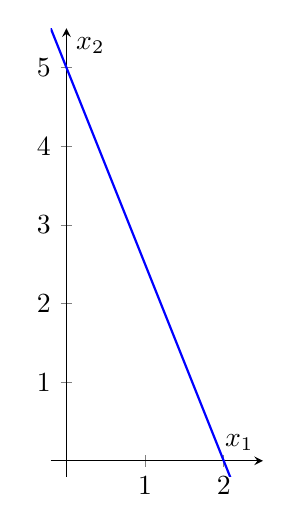
\begin{tikzpicture}
		\begin{axis}[
			xlabel=$x_1$,
			ylabel=$x_2$,
			axis equal image,
			axis lines=middle,
			xtick={0,1,...,2},
			ytick={0,1,...,5},
			xmin=-0.2,
			ymin=-0.2,
			xmax=2.5,
			ymax=5.5,
			]
			\addplot[color=blue, thick]{-5/2 * x + 5};
		\end{axis}
	\end{tikzpicture}
\end{center}
General form of this linear classifier:
\begin{align*}
	y_k = W^T X + b
\end{align*}
With $W$ being the normal vector of the two-dimensional hyperplane (line) going through $s_1=(0,5)$ and $s_2=(2,0)$:
\begin{align*}
	W^T &= 
	\begin{pmatrix}
	dx_2\\-dx_1
	\end{pmatrix}^T
	\quad\quad with\quad dx_1 = 0 - 2 = -2\quad,\ dx_2= 5-0 = 5\\
	&= 
	\begin{pmatrix}
	5\\2
	\end{pmatrix}^T
\end{align*}
The bias can be computed by inserting a point on the plane (e.g. $s_2$) and setting the classifier to $0$, like this:
\begin{align*}
	b = 0 - W^T X = 0 - 
	\begin{pmatrix}
	5 & 2
	\end{pmatrix}
	\begin{pmatrix}
	2\\0
	\end{pmatrix}
	= -10
\end{align*}
The classifier with some possible parameters is therefore:
\begin{align*}
	y_k = 
	\begin{pmatrix}
	5\\2
	\end{pmatrix}^T 
	X - 10
\end{align*}

\pagebreak

\exercise
\begin{lstlisting}[language=Python]
	def pred(X, W, b):    
	    c = np.add(b, np.dot(X, W.transpose()))
	    
	    if np.isscalar(c):
	        c = np.array([c])
		
	    for x in np.nditer(c, op_flags=['readwrite']):
		    # transform each position with 1 / (1 + exp(-a))
		    x[...] = 1 / (1 + np.exp(-1 * x))
		
	    return np.reshape(c, (X.shape[0],1))
\end{lstlisting}

\exercise
\begin{lstlisting}[language=Python]
	def loglikelihood(X, Z, W, b):    
	    error = 0
	    for i in range(X.shape[0]):
		    error += Z[i] * np.log(pred(np.array([X[i]]), W, b))
	                  + (1 - Z[i]) * np.log(1 - pred(np.array([X[i]]), W, b))    
	    return error
\end{lstlisting}

\end{document}